\documentclass[11pt]{article}
\input{/Users/markwang/.preamble}
\begin{document}



% arg1=pdfurl arg2=pagenum arg3=sectiontitle
\newcommand{\linksection}[3][../../bishop_pattern_recognition_and_machine_learning.pdf]{
    \subsection*{\href[page=#2]{#1}{#3}}
}

\newcommand{\linkinline}[3][../../bishop_pattern_recognition_and_machine_learning.pdf]{
    \noindent\href[page=#2]{#1}{#3}
}

\renewcommand{\norm}[1]{\left\lVert#1\right\rVert}
\renewcommand{\E}[2][]{\mathbb{E}_{#1}\left\{#2\right\}}
\newcommand{\var}[2][]{var_{#1}\left\{#2\right\}}
\newcommand{\cov}[1]{cov\{#1\}} 
\newcommand{\normal}[1]{\mathcal{N}\left(#1\right)}
\newcommand{\exponents}[1]{exp\left\{#1\right\}}

\newcommand{\bmu}{\boldsymbol{\mu}}
\newcommand{\bpi}{\boldsymbol{\pi}}
\newcommand{\bTheta}{\boldsymbol{\Theta}}
\newcommand{\bSigma}{\boldsymbol{\Sigma}}
\newcommand{\bphi}{\boldsymbol{\phi}}

\newcommand{\calL}{\mathcal{L}}
\newcommand{\calE}{\mathcal{E}}
\newcommand{\calR}{\mathcal{R}}
\newcommand{\calC}{\mathcal{C}}
\newcommand{\calD}{\mathcal{D}}
\newcommand{\bx}{\matr{x}}
\newcommand{\bt}{\matr{t}}
\newcommand{\bw}{\matr{w}}
\newcommand{\bX}{\matr{X}}
\newcommand{\bZ}{\matr{Z}}
\newcommand{\bz}{\matr{z}}
\newcommand{\bu}{\matr{u}}



\newcommand{\lebpar}[2]{\frac{\partial #1}{\partial #2}}
\newcommand{\qqqquad}{\quad \quad \quad \quad}

\newcommand{\condi}[3]{#1 \Vbar #2 \,|\, #3}
\newcommand{\notcondi}[3]{#1 \not\Vbar #2 \,|\, #3}


\linksection{538}{11 Sampling Methods} 

\begin{defn*}
    \textbf{Sampling}
    \begin{enumerate}
        \item \textbf{Motivation} Approximate inference methods on models where exact inference is intractable. We consider approximate inference based on numerical sampling, i.e. Monte Carlo stuff
        \item \textbf{Goal} Computing expectation of some function $f(\bz)$ with respect to some probability distribution $p(\bz)$ which is usually too complex to be evaluated analytically
        \[
            \E{f} = \int f(\bz) p(\bz) d\bz    
        \]
        \item \textbf{Approach} Obtain a set of samples $\bz^{(l)}$ where $l=1,\cdots, L$ drawn independently from distribution $p(\bz)$. We then approximate the expectation by a finite sume 
        \[
            \hat{f} = \frac{1}{L} = \sum_{l=1}^L f(\bz^{(l)})   
            \qquad \textbf{where} \qquad 
            \E{\hat{f}} = \E{f} 
            \quad 
            \var{\hat{f}} = \frac{1}{L} \var{f}
        \]
    \end{enumerate}
\end{defn*}



\begin{defn*}
    \textbf{Baysian Monte Carlo}
    \begin{enumerate}
        \item \textbf{Goal} Want to approximate $\E[\theta \sim p(\theta)]{f(\theta)}$. But we cannot compute $p(\theta)$ directly, instead we can compute $g = \textstyle \frac{p}{c}$ for some normalizing constant $c$. We want to find 
        \[ 
            \E{f} = \frac{\int f(\theta) g(\theta) d\theta}{\int g(\theta) d\theta}    
        \]
        \item \textbf{Idea} Generate a set of samples $\{\ \theta_i \,\, \}_{i=1}^N$ from $p(\theta)$ and 
        \[
            \E{f} \simeq  \frac{1}{N} \sum_{i=1}^Nf(\theta_i)
        \]
        \item \textbf{Context of Bayesian} $f$ is the prediction. $p$ is some posterior distribution we cannot evaluate directly. $g = p(\mathcal{D} | \theta) p(\theta)$ is product of prior and likelihood which is computable, we can then sample 
        \[  
            p = p(\theta | \mathcal{D}) \overset{bayes}{=}
            \frac{p(\mathcal{D} | \theta) p(\theta)}{\int p(\mathcal{D} | \theta) p(\theta) d\theta}
            = \frac{g(\theta)}{\int g(\theta)d\theta}
            = \frac{g}{c}
            \qquad c\in \R
        \]
        In this case the estimator is unbiased and variance shrinks by a factor of sample size
        \[
            \E[\theta \sim p]{\hat{f}(\theta)} = \frac{1}{N} \sum_{i=1}^N \E[\theta \sim p]{f(\theta)} = \E[\theta\sim p]{f(\theta)}
        \]
        \[
            \var[\theta \sim p]{\hat{f}(\theta)} = \frac{1}{N^2} \sum_{i=1}^N \var[\theta \sim p]{f(\theta)} = \frac{1}{N}\var[\theta\sim p]{f(\theta)}
        \]
    \end{enumerate}
\end{defn*}


\begin{defn*}
    \textbf{Ancestral Sampling} \linkinline{381}{(8.1.2)}
    \begin{enumerate}
        \item \textbf{Idea} Sample $\hat{x}_1, \cdots, \hat{x}_K$ from a joint distribution $p(x_1, \cdots, x_K)$ which factorizes into a directed acyclic graph. 
        \item \textbf{Algorithm} Order varaibles such that they follow topological ordering. Start with drawfing a sample $\hat{x}_1$ from distribution $p(x_1)$, then work through each node in oder such that for node $x_i$, we draw sample from $p(x_i | parent(x_i))$, where the parent variables are set to sampled values. 
        \item \textbf{Summary} We make one pass through set of variables in order $\bz_i , \cdots, \bz_M$, by sampling from conditional distribution $p(\bz_i | parent(\bz_i))$ where 
        \[
            p(\bz)=  \prod_{i} p(\bz_i | parent(\bz_i))    
        \]
    \end{enumerate}
\end{defn*}


\begin{defn*}
    \textbf{Sampling from standard distribution} Given $z \sim p(z)$ we want to determine a function $f(\cdot)$ such that $y = f(z)$ is a desired distribution. The following relationship holds
    \[
        p(y) = p(z) \left| \frac{dz}{dy} \right|    
    \]
    We usually want to convert a pseudo-random number generator with uniform distribution $[0,1]$ to a desired distribution. So $p(z) = 1$, goal is to pick $f$ by integration
    \[
        f = h^{-1}
        \qquad 
        z = h(y) = \int_{-\infty}^y p(y) dy
    \]
    This method has the limitation that it requires inverting a indefinite integral and that we are able to sample from $p(z)$
\end{defn*}

\begin{defn*}
    \textbf{Rejection Sampling} \\ 
    Given we cannot sample from $p(\bz)$ directly. But we do have 
    \begin{enumerate}
        \item \textbf{A readily computable function} $\tilde{p}(z)$, such that $p(z) = \textstyle\frac{1}{Z} \tilde{p}(z)$. 
        \item \textbf{A proposal distribution} $q(z)$, from which we can sample easily 
    \end{enumerate}
    that satisfies the inequality $kq(z) \geq \tilde{p}(z)$
    \begin{center}
        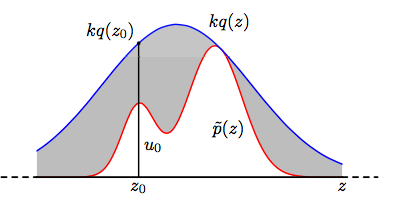
\includegraphics[width=6cm]{rejection_sampling.png}
    \end{center}
    We generate $z_0 \sim q(z)$ and $u_0 \sim Unif[0, kq(z_0)]$. We reject sample $z_0$ if $u_0 > \tilde{p}(z_0)$ otherwise accept the sample. In this way, the accepted samples falls uniformly under the curve of $\tilde{p}(z)$, and hence the corresponding accepted samples are distributed according to $p(z)$. Note rejection sampling rejects exponentially more samples (hence inefficient) for high dimensional distributions. It also has problem with picking the right $k$ and a good upper bound distribution $q$. 
\end{defn*}


\begin{defn*}
\textbf{Metropolis-Hasting Algorithm} We want to maintain a record of current state $\bz^{\tau}$ and the proposal distribution $q(\bz | \bz^{(\tau)})$ depends on the current state. A sequence $\{\bz^{(1)}, \bz^{(2)}, \cdots \}$ forms a markov chain. Again we want to sample from $p(\bz) = \textstyle \frac{\tilde{p}{\bz}}{c}$ for some $c\in \R$. At each iteration of the algorithm, we generate candidate $\bz^* \sim q(\bz| \bz^{(\tau)})$ and accept the sample with probability 
    \[
        A(\bz^*, \bz^{(\tau)}) = \min \left( 1, \frac{\tilde{p}(\bz^*) q(\bz^{(\tau)}| \bz^*)  }{\tilde{p}(\bz^{(\tau)}) q(\bz^* | \bz^{(\tau)})} \right)
    \]
    this can be achieved by choosing a random number $u\sim Unif(0,1)$ and accpet the sample if $A(\bz^*, \bz^{(\tau)}) > u$. In general, the algorithm favors accepting samples with 
    \begin{enumerate}
        \item $\tilde{p}(\bz^*) \geq \tilde{p}(\bz^{(\tau)})$, i.e. if transition yields higher value of $p(\bz)$
        \item $q(\bz^{(\tau)}| \bz^*) \geq q(\bz^* | \bz^{(\tau)})$, i.e. if current state is easier to get back to
    \end{enumerate}
    We can prove that distribution of $\bz^{(\tau)}$ tends to $p(\bz)$ as $\tau \rightarrow \infty$. Notice, the proposal distribution is not that important, as the long term convergence is guaranteed
\end{defn*}

 
\end{document}
